\documentclass{article}

%Packages
\usepackage[utf8]{inputenc} % encoding

\usepackage[margin=1in]{geometry} % Wide paper format
\usepackage[colorlinks]{hyperref} % Links and references 
\usepackage{setspace} % Double-/single spacing
\usepackage{graphicx} % Figures
\usepackage{subcaption} % Subfigures
\usepackage{rotating} % Sideways table
\usepackage{pgfplotstable} % Generates table from .csv
\usepackage{smartdiagram} % Generate easy diagrams
\usepackage{amsmath} %math

%Titlepage
\title{A short abstract on hummingbirds}
\date{04-09-2018}
\author{Charles Darwin}


\begin{document}
%Titlepage and TOC
\maketitle
\tableofcontents
\newpage

%Set formatting
\doublespacing
\setlength\parindent{0pt}
\section{First Section: Links and hyperrefs}
This is a first section. You can add links: \url{https://www.latex-tutorial.com/}. And give them a name:
\href{https://www.latex-tutorial.com/}{LatexTutorial}.
\subsection{Subsection}
This is a useless subsection.
\section{Second Section: Lists and enumerations}
\begin{minipage}[t]{0.3\textwidth}
\singlespacing
My List:
\begin{itemize}
	\item[-] one
	\item[*] two
	\item[???] three
\end{itemize}
\end{minipage}
\begin{minipage}[t]{0.3\textwidth}
\singlespacing
My enumeration:
\begin{enumerate}
	\item first
	\item second
	\item third
\end{enumerate}

\bigskip
\end{minipage}



\section{Third Section: Figures and Floats}
We are investigating hummingbirds (Figure \ref{bird}).

\begin{figure}[h]
	\centering
	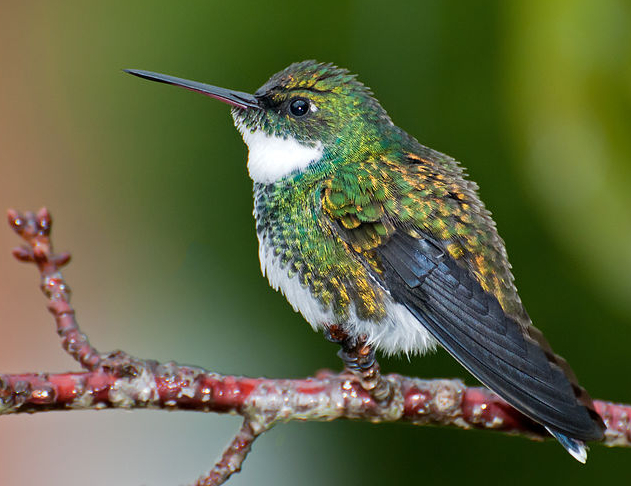
\includegraphics[scale=1]{bird.jpg}
	\caption{A humming bird?}
	\label{bird}
\end{figure}

%Good website for floats and figures:
%https://en.wikibooks.org/wiki/LaTeX/Floats,_Figures_and_Captions

\begin{figure}[h]
  \centering
  \begin{subfigure}[b]{0.5\linewidth}
    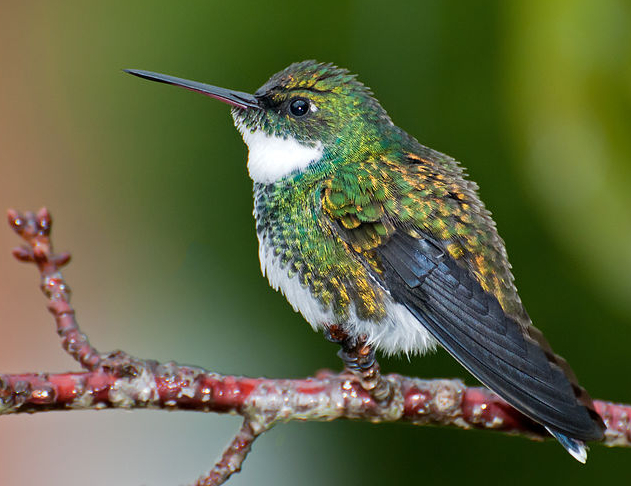
\includegraphics[width=\linewidth]{bird.jpg}
    \caption{A humming bird?}
  \end{subfigure}
  \\
  \begin{subfigure}[b]{0.3\linewidth}
    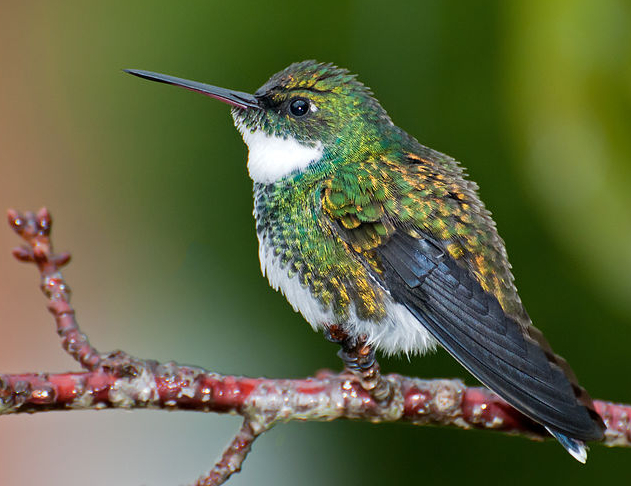
\includegraphics[width=\linewidth]{bird.jpg}
    \caption{Another humming bird?}
  \end{subfigure}
  \begin{subfigure}[b]{0.3\linewidth}
    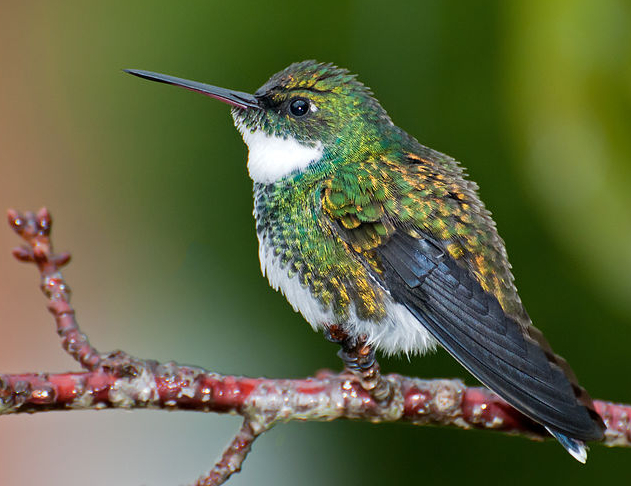
\includegraphics[width=\linewidth]{bird.jpg}
    \caption{Another humming bird?}
  \end{subfigure}
  \begin{subfigure}[b]{0.3\linewidth}
    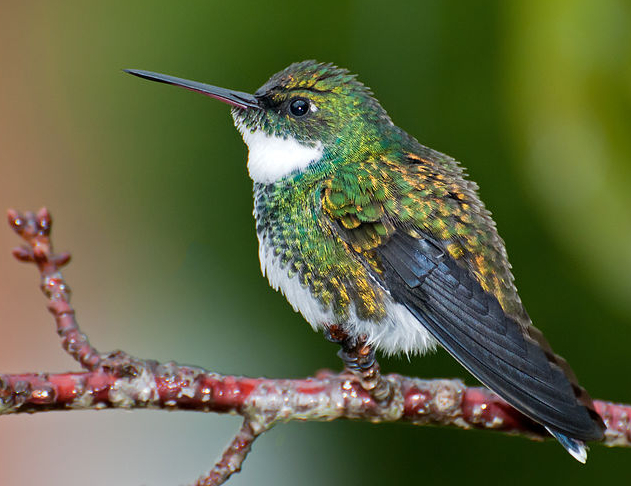
\includegraphics[width=\linewidth]{bird.jpg}
    \caption{Another humming bird?}
  \end{subfigure}
  \caption{The same "humming" bird multiple times.}
  \label{rats}
\end{figure}


Quisque nec nunc lobortis, mattis massa ac, blandit neque. Proin eget lacus diam. In in libero eu velit suscipit suscipit quis non enim. Donec at ipsum eros. Nulla nunc odio, dapibus a arcu nec, ornare rutrum quam. Aliquam purus metus, lacinia vel arcu a, interdum mattis ante. Aenean neque augue, congue egestas lectus quis, consectetur interdum massa. Proin diam libero, tincidunt id sodales elementum, bibendum at nulla. Class aptent taciti sociosqu ad litora torquent per conubia nostra, per inceptos himenaeos. Morbi laoreet elit mi, ac finibus felis tempus vitae. Donec in congue nisi. Praesent viverra bibendum pellentesque. In rutrum sem efficitur consequat vehicula. Cras aliquam arcu dolor, at aliquet nibh hendrerit sit amet.


\section{Citations}
%http://rsif.royalsocietypublishing.org/content/11/99/20140585
%http://www.bioinformatics.org/texmed/
Hummingbird wing efficacy similar to helicopter rotors \cite{Kruyt20140585}.


\section{Tables}

%Simple table 
\begin{table}[h!]
  \begin{center}
    \caption{Your first table.}
    \label{table1}
    \begin{tabular}{l|c|r} % <-- Alignments: left,center,right, with vertical lines in between
      \textbf{first col} & \textbf{second col} & \textbf{third col}\\
      \hline
      1 & I & a\\
      2 & II & b\\
      3 & III & c\\
    \end{tabular}
  \end{center}
\end{table}

%
Tired of typing your tables? \url{https://www.tablesgenerator.com/}

%Import table from file
\begin{table}
\centering
\caption{Autogenerated table from .csv file.}
\label{table1}
\pgfplotstabletypeset[col sep=comma,string type]{table.csv}
\end{table}

\section{Math}

$f(x) = x^2$


\section{Diagrams}
%Diagrams
Smart Diagram package: \url{http://latex-cookbook.net/articles/smart-diagrams/}

\vspace{20pt}

\centering
\smartdiagram[flow diagram:horizontal]{Edit,
  \LaTeX, Bib\TeX/ biber, make\-index, \LaTeX}

\bigskip

\begin{center}
\smartdiagram[descriptive diagram]{
      {Style,{Define shapes, colors, shading,
              and line styles for nodes and arrows}},
      {Position, {Place nodes using a matrix,
                  relative or absolute positioning}},
      {Relation, Insert edges or arrows
                 between selected nodes},
      {Label, Add labels on edges or arrows}}
\end{center}
% List of figures/tables
\newpage

\begin{appendix}
  \listoffigures
  \listoftables
\end{appendix}

%Bibtex references 
%http://www.bioinformatics.org/texmed/
\bibliography{references} 
\bibliographystyle{plain}
\end{document}
